% Chapter 3: Project Development

\chapter{Desarrollo del Proyecto} % Main chapter title

\label{Chapter3} % For referencing this chapter elsewhere, use \ref{Chapter3}

%-------------------------------------------------------------------------------

\section{Trabajo previo}

%-------------------------------------------------------------------------------

\section{Arquitectura del software}

El objetivo de este proyecto es proporcionar un servicio que permita analizar proyectos \emph{software}\index{software} de una manera sencilla y automatizada. Para ello, se ha llevado a cabo el desarrollo de varios prototipos:

\begin{itemize}
    \item El primer prototipo sienta las bases de la arquitectura de la aplicación. La API\index{API} consta de algunas llamadas básicas para la creación de solicitudes de análisis y el cliente es capaz de procesarlas y retornar este resultado al usuario.
    \item El segundo prototipo añade \nameref{sec:grimoirelab}\index{GrimoireLab} y \nameref{sec:opensearch}\index{OpenSearch} al esquema de la aplicación. La API\index{API} incluye nuevas estructuras y llamadas y el cliente ejecuta tareas de análisis con GrimoireLab y sube los resultados a OpenSearch para su visionado.
\end{itemize}

\subsection{Grimoirebots I}

El primer prototipo de la aplicación está creado utilizando el framework Django REST Framework para Python, y Poetry como gestor de paquetes y dependencias. Esta primera versión establece la arquitectura base de la aplicación y el esquema de comunicación entre servidor y cliente.

Para este fin, se han desarrollado los siguientes modelos:

\begin{figure}[ht]
    \centering
    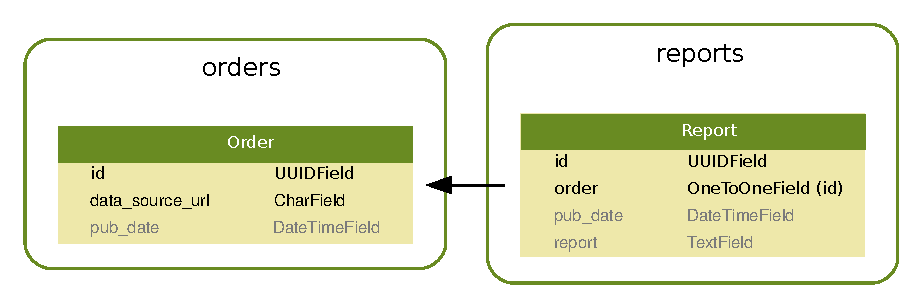
\includegraphics[width=0.8\textwidth]{Figures/grimoirebots_i_models}
    \decoRule
    \caption[Grimoirebots I (modelos)]{Modelos usados en Grimoirebots (Versión 1)}
    \label{fig:grimoirebots_i_models}
\end{figure}

\begin{itemize}
    \item \code{Order} -- Este modelo representa la solicitud hecha por un usuario. Está formado por un identificador UUID único, un \emph{string} representando la URL del repositorio git que se quiere analizar, y la fecha de creación de la instancia con un campo \emph{datetime}.
    \item \code{Report} - Este modelo representa el resultado de procesar una solicitud hecha por un usuario. Está formado por un identificador UUID único, una referencia a la solicitud (\code{Order}) que originó su creación, la fecha de creación de la instancia con un campo \emph{datetime}, y un \emph{string} representando el procesamiento de la solicitud.
\end{itemize}

- Esquema básico
- Recibe el input del usuario y crea estructuras básicas con este
- Crea reports en los que solo hay texto
- Tiene el endpoint para recoger las tareas sin report
- Uso de DRF
- Dockerfile
- Sqlite
- Dependabot

\subsection{Grimoirebots II}

\begin{figure}[ht]
    \centering
    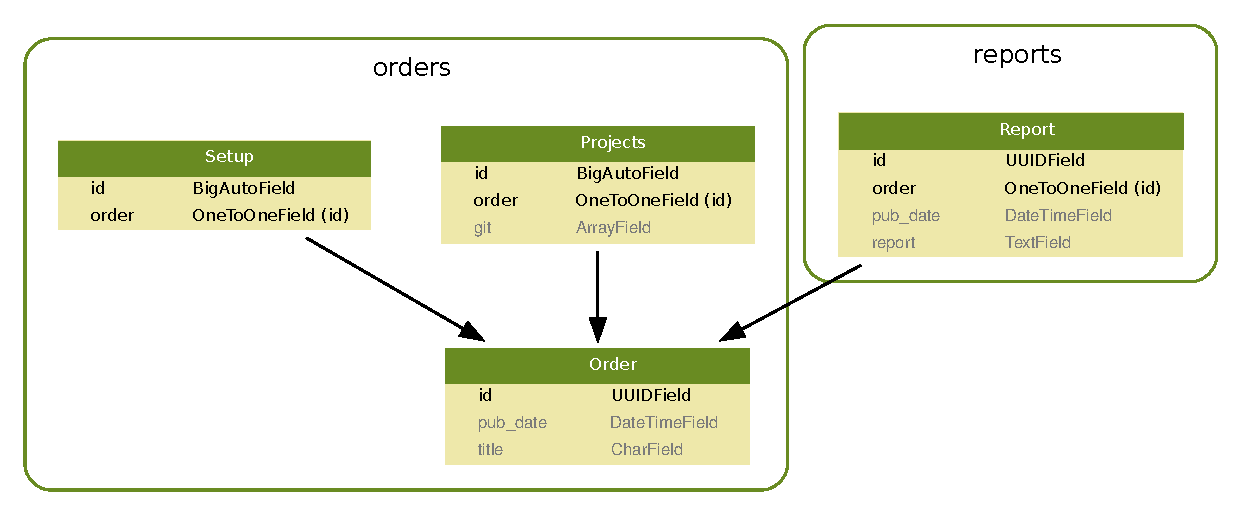
\includegraphics[width=0.8\textwidth]{Figures/grimoirebots_ii_models}
    \decoRule
    \caption[Grimoirebots II (modelos)]{Modelos usados en Grimoirebots (Versión 2)}
    \label{fig:grimoirebots_ii_models}
\end{figure}

- Inclusión de los modelos Projects y Setup
- Inclusión de OpenSearch
- Inclusión de GrimoireLab
- Inclusión de la OpenAPI spec en la app
- Inclusión de PostgreSQL
- Unificación de endpoints para project y setup

\subsection{Grimoirebots client I}

Bot que recoge las órdenes pendientes y crea un elemento report con un texto

\subsection{Grimoirebots client II}

- Bot que recoge las ordenes pendientes y lanza un contenedor de Docker con GrimoireLab
- El cliente crea los volúmenes de donde los contenedores recogen la información

%-------------------------------------------------------------------------------

\section{Problemas encontrados}

- Se tuvo que eliminar la inclusión de usuarios debido a la complejidad que añadía al sistema, y debido a que el tiempo dedicado no era suficiente.

- Demasiada ambición en los primeros prototipos, eso hizo que se ralentizara el desarrollo inicial.

- Se quiso usar en un principio Django, con sus templates, con un front-end, etc. Se decidió usar DRF por sus serializers, en conjunto con las templates de Django, pero estas no casaban muy bien. Esto causó bastante pérdida de tiempo.

- GrimoireLab no soporta las versiones más modernas de OpenSearch.

- Falta de conocimiento sobre los estudios de GrimoireLab

- Lanzar contenedores desde un contenedor fue algo complicado.

- Realizar el TFM a la vez que un trabajo que demanda mucho tiempo y esfuerzo.

- Se quiso incluir paginación, pero se descartó por la complejidad que luego suponía en el cliente.

- El envío del fichero setup.cfg fue un problema debido al formato. Al no ser JSON, DRF no lo podía devolver directamente. Se probaron varias cosas hasta que se decidió devolverlo en JSON y que fuera el cliente el que lo tradujera al formato necesario.

- Se intentó realizar una comparativa entre DRF y FastAPI, pero se descartó por falta de tiempo. Se consiguió crear una versión muy básica de Grimoirebots, pero no funcional.
